\subsection{Memcached-silo}
\label{sec:mcdsilo}

Memcached-silo is a workload built on top of the normal memcached protocol. It is computationally and memory more intensive than regular memcached as it incorporates both latency-sensitive network compute and memory-intensive TPC-C style transaction processing. The workload is structured such that every single memcached request triggers a corresponding set of fixed TPC-C transaction processing logic on a in-memory database~\cite{silo}. We ported the memcached-silo implementation~\cite{mcdsilo, zygos} to our libOS. The workload mix and SLA constraints of memcached-silo follow from those used in the memcached experiments. Given its computationally heavier nature, we only needed two 16-core client nodes at 16 connections per core to saturate a single 16-core memcached-silo server. 

\begin{figure*}
\centering
%\vspace*{-0.3cm}  
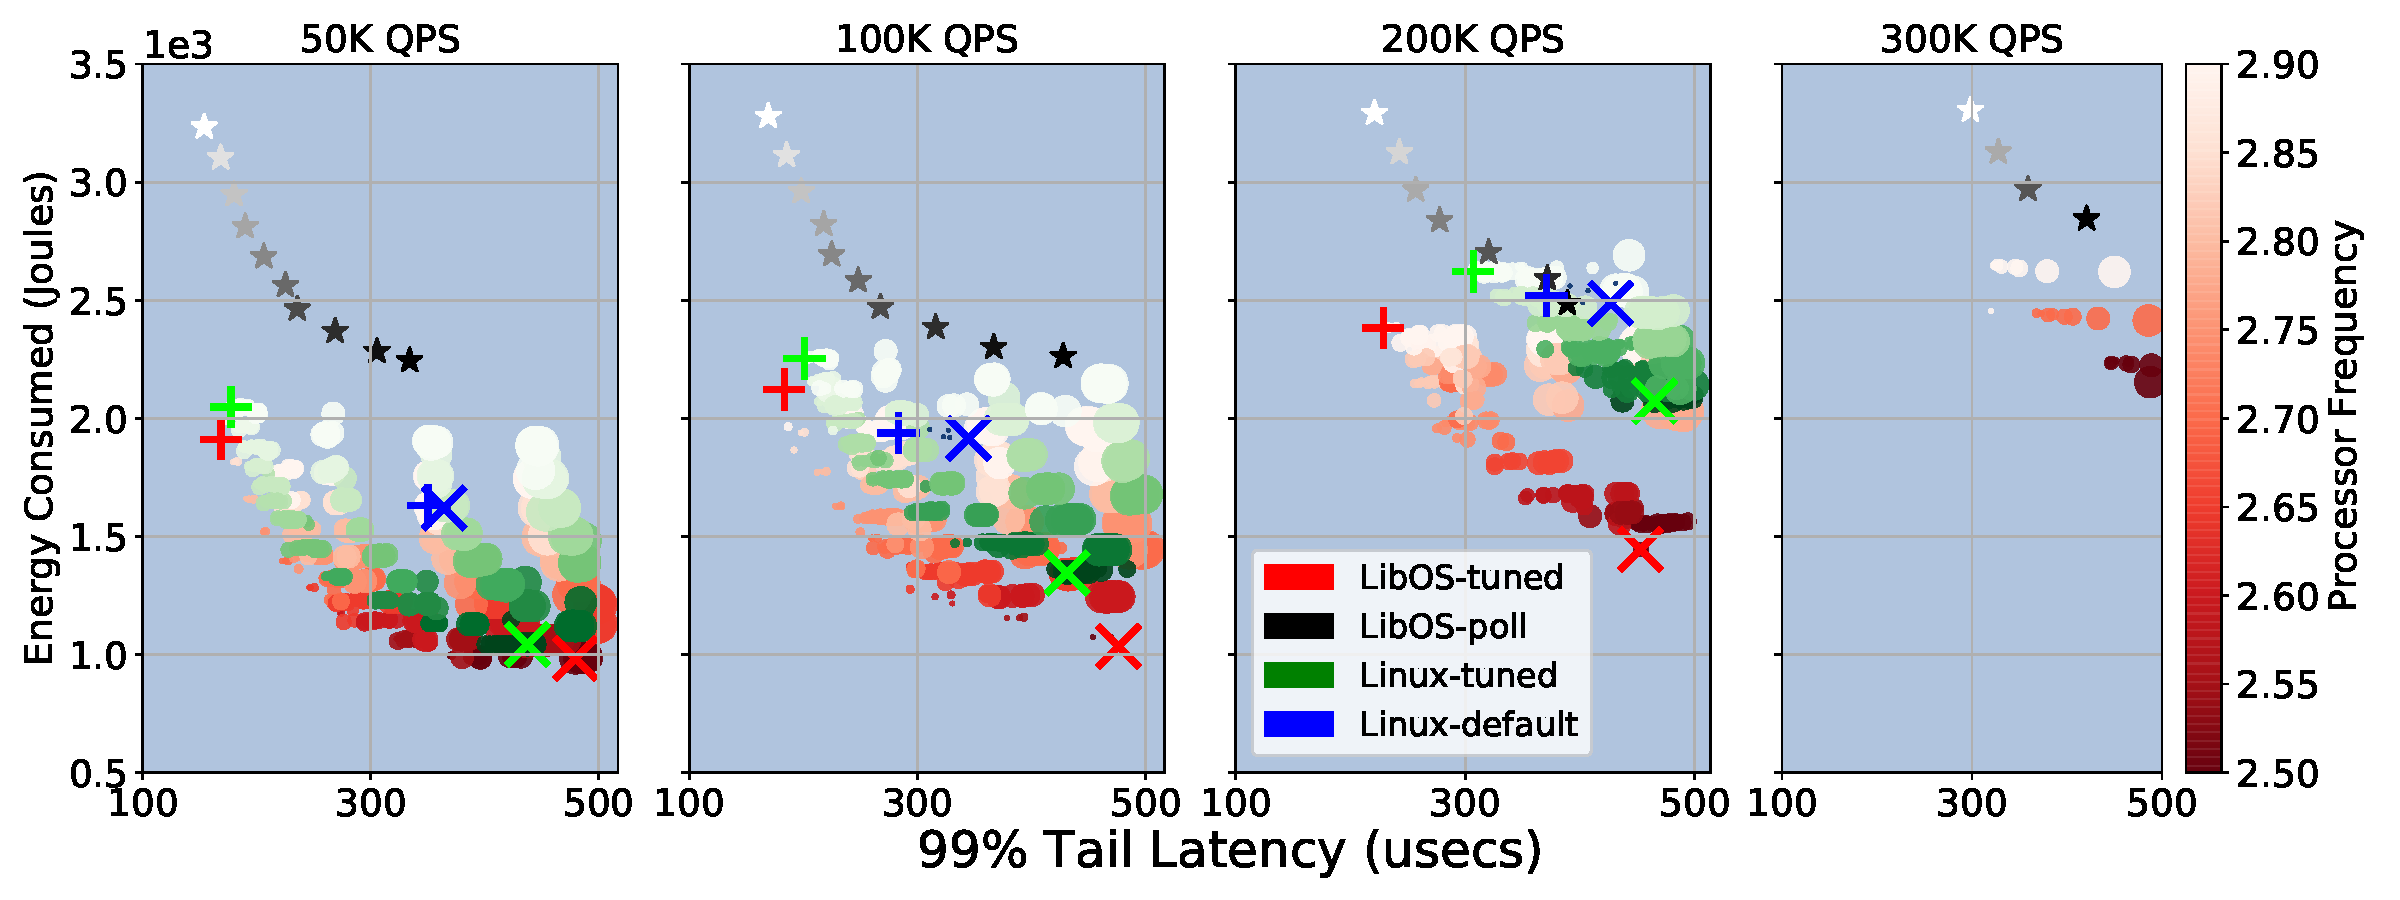
\includegraphics[width=1\textwidth]{figures/mcdsilo_overview}
\caption[]
%{\small 
{Memcached-silo across different QPS.}
\label{fig:mcdsilo_overview}
\end{figure*}

\begin{figure}
%\centering
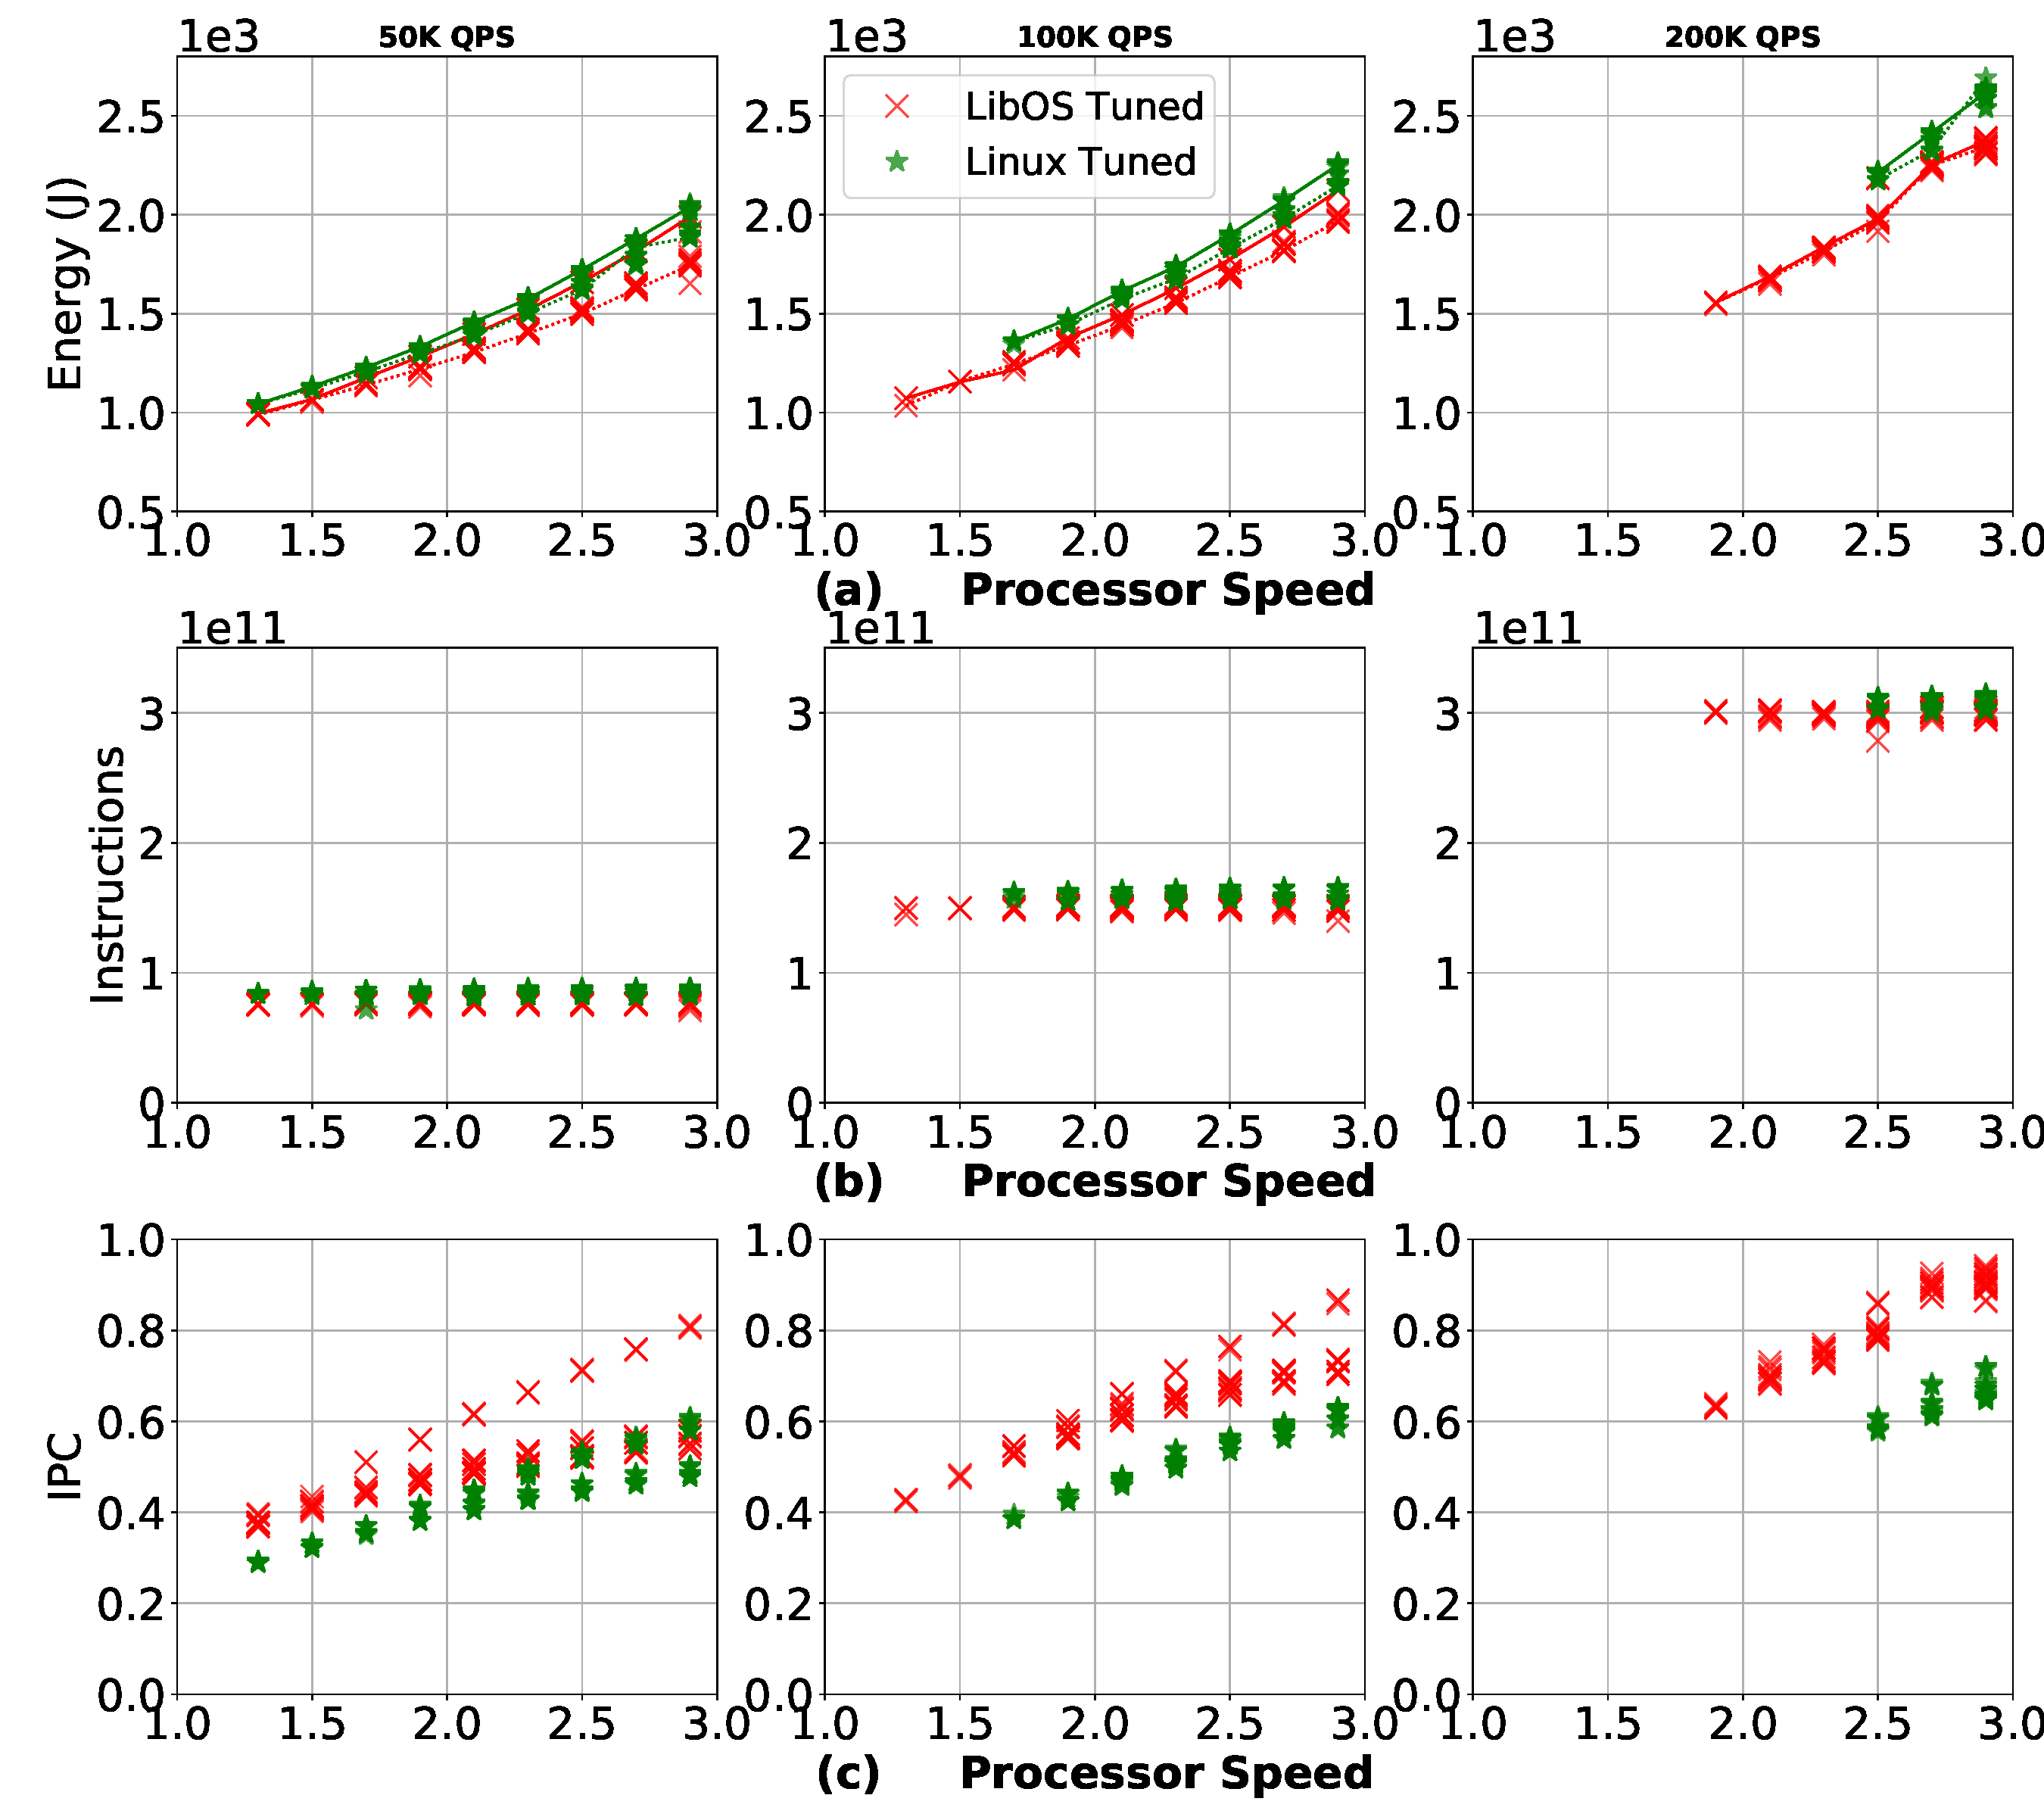
\includegraphics[width=0.5\textwidth]{figures/mcdsilo_detail}
%\hspace*{-10.0cm} 
%\vspace*{-1.0cm}  
\caption[]{}
\label{fig:mcdsilo_detail}
\end{figure}

\subsubsection{Finding-1: Implications of OS path length efficiency}

% ebbrt_tuned c1 4 0x1d00 135    159.0 1954.58
% ebbrt_tuned c1e 4 0x1d00 135   203.1 1789.93
% ebbrt_tuned c3 4 0x1d00 135    205.2 1779.41
% ebbrt_tuned c7 4 0x1d00 135    206.0 1789.72
% ebbrt_tuned c1 200 0xd00 135   471.5 991.89
% ebbrt_tuned c1e 200 0xd00 135  483.5 990.82
% ebbrt_tuned c3 200 0xd00 135   488.0 987.11
% ebbrt_tuned c7 200 0xd00 135   488.4 989.57

% ebbrt_tuned c1 2 0x1d00 135 304.2 2631.54
% ebbrt_tuned c1e 2 0x1d00 135 312.0 2637.85
% ebbrt_tuned c3 2 0x1d00 135 322.5 2631.96
% ebbrt_tuned c7 2 0x1d00 135 326.9 2646.27

% ebbrt_tuned c1 100 0x1900 135 481.8 2210.25
% ebbrt_tuned c1e 100 0x1900 135 486.1 2051.88
% ebbrt_tuned c3 100 0x1900 135 491.8 2209.09
% ebbrt_tuned c7 100 0x1900 135 492.4 2214.79

% \begin{table}[t]
% \centering
% \begin{tabular}{l|c|c|c|c|c|}
%   QPS & Type & Sleep State & Latency (\SI{}{\micro s}) & Energy (\SI{}{\joule})\\ \hline
%   50K & Min-Tail & C1 & 159 & 1954\\ \hline
%   50K & Min-Tail & C1E & 203 & 1789\\ \hline
%   50K & Min-Tail & C3 & 205 & 1779\\ \hline
%   50K & Min-Tail & C7 & 206 & 1789\\ \hline
%   50K & Min-Energy & C1 & 471 & 991\\ \hline
%   50K & Min-Energy & C1E & 483 & 990\\ \hline
%   50K & Min-Energy & C3 & 488 & 987\\ \hline
%   50K & Min-Energy & C7 & 488 & 989\\ \hline
%   300K & Min-Tail & C1 & 304 & 2631\\ \hline
%   300K & Min-Tail & C1E & 312 & 2637\\ \hline
%   300K & Min-Tail & C3 & 322 & 2631\\ \hline
%   300K & Min-Tail & C7 & 326 & 2646\\ \hline
%   300K & Min-Energy & C1 & 481 & 2210\\ \hline
%   300K & Min-Energy & C1E & 486 & 2207\\ \hline
%   300K & Min-Energy & C3 & 491 & 2209\\ \hline
%   300K & Min-Energy & C7 & 492 & 2214\\ \hline
% \end{tabular}
% \caption{Min-Tail refers to configuration of processor speed and interrupt rate where the lowest tail latency was achieved and Min-Energy refers to the configuration with lowest energy use.}
% %\caption{Workload configurations.
% %The column {\em Nature} indicates open-versus-closed loop nature
% %and {\em CPU} indicates application CPU demand.}
% \label{table:mcdsilo_sleep_states}	
% \end{table}
\subsubsection{Finding-1: Implications of OS path length efficiency}
